\chapter{Implementacja}
\label{cha:impl}

Mając do dyspozycji układ heterogeniczny rodziny Zynq-7000 od firmy Xilinx operacje zostały podzielone między programowalną logiką a systemem procesorowym. Ogólny zarys systemu został przedstawiony na rysunku \ref{fig:systemwizyjny}.

\begin{figure}[h]
    \centering
    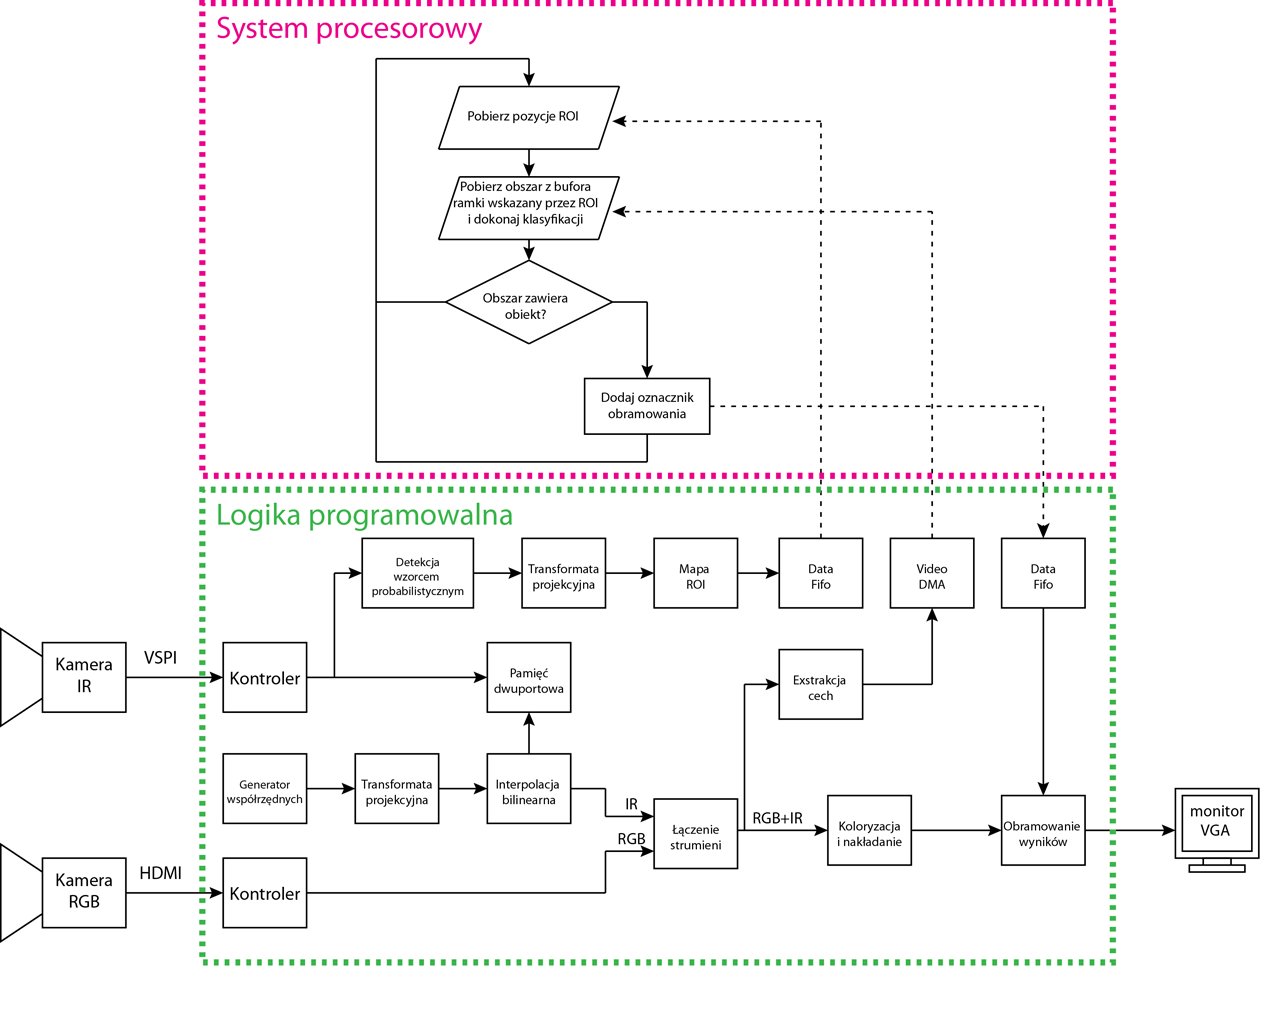
\includegraphics[width=1\textwidth]{images/system}
    \caption{Schemat blokowy systemu detekcji.}
    \label{fig:systemwizyjny}
\end{figure}

Programowalna logika:
\begin{itemize}
\item Akwizycja Obrazu poprzez HDMI (RGB) i VoSPI (IR),
\item Transformata projekcyjna i interpolacja obrazu IR,
\item Nałożenie i synchronizacja obrazu IR do obrazu RGB,
\item Ekstrakcja cech z połączonych obrazów,
\item Prezentacja wyników,
\item Detekcja kandydatów za pomocą wzorca probabilistycznego.
\end{itemize}
System Procesorowy:
\begin{itemize}
\item konfiguracja parametrów systemu wizyjnego w logice programowalnej poprzez interfejs AXI-Lite,
\item Klasyfikacja obszarów wytypowanych przez wzorzec probabilistyczny,
\item Generowanie oznaczników.
\end{itemize}

\section{Opis modułów}

\subsection{Transformata projekcyjna}
Zadaniem modułu jest dostosowanie obrazu IR by pokrywał się z obrazem RGB. Moduł transformaty projekcyjnej zamienia wygenerowane współrzędne w zakresie wielkości przychodzącego obrazu RGB na odpowiadające im punkt na obrazie IR (wraz z częścią ułamkową). Moduł jest konfigurowalny poprzez interfejs AXI-Lite, za pomocą którego można ustawić wartość minimalną i maksymalną współrzędnych wyjściowych U i V oraz macierz transformaty.
\subsection{Kontroler kamery IR}
Pobiera obraz z kamery poprzez interfejs VoSPI który następnie zostaje zapisany do dwuportowej pamięci BRAM.
\subsection{Interpolacja bilinearna}
Prosty moduł przeznaczony głównie do powiększania obrazów. Pobiera wartość 4 otaczających, podanych na wejściu punktu, pikseli z BRAM i na ich bazie jest wykonywana interpolacja. Moduł zapamiętuje 4 ostatnio użyte piksele które są na bieżąco aktualizowane wraz z zmianą położenia punktu wejściowego na obrazie IR.
\subsection{Łączenie strumieni}
Moduł posiada dwa wejścia dla obrazu. Jeden strumień jest głównym i do niego jest dołączany drugi strumień. Do synchronizacja strumieni została wykorzystana możliwość AXI-Strem do wstrzymania transmisji. Piksele z dołączanego strumienia są odrzucane do momentu pojawienia się sygnału SOF. W momencie pojawienia się sygnału SOF w strumieniu głównym transmisja zostaje wznowiona pod kontrolą strumienia wyjściowego. 
\subsection{Koloryzacja i nakładanie}
Połączone strumienie RGB+IR zostają połączone w jeden obraz. Obraz IR zostaje poddany koloryzacji na podstawie 12-bitowego LUT i nałożony w proporcjach 50 na 50 z obrazem RGB.
